% Detaillierte Beschreibung bestimmter für das Programm wichtige Abläufe anhand von Sequenzdiagrammen. Es sollten etwa 3-4 charakteristische und interessante Abläufe ausgewählt werden.
\section{Crawler}
\subsection{Start des Crawlers}
Beim Starten des Crawlers werden sämtliche notwendigen Komponenten der Reihe nach gestartet. Dadurch wird garantiert, dass jede Komponente eine Umgebung vorfindet in der sie laufen kann und alle Ressourcen bereits zur Verfügung stehen. In \cref{fig:crawler_start} ist der Start des Crawlers beispielhaft mit 2 StatusProcessor's dargestellt.
\begin{figure}[h!]
	\centering
	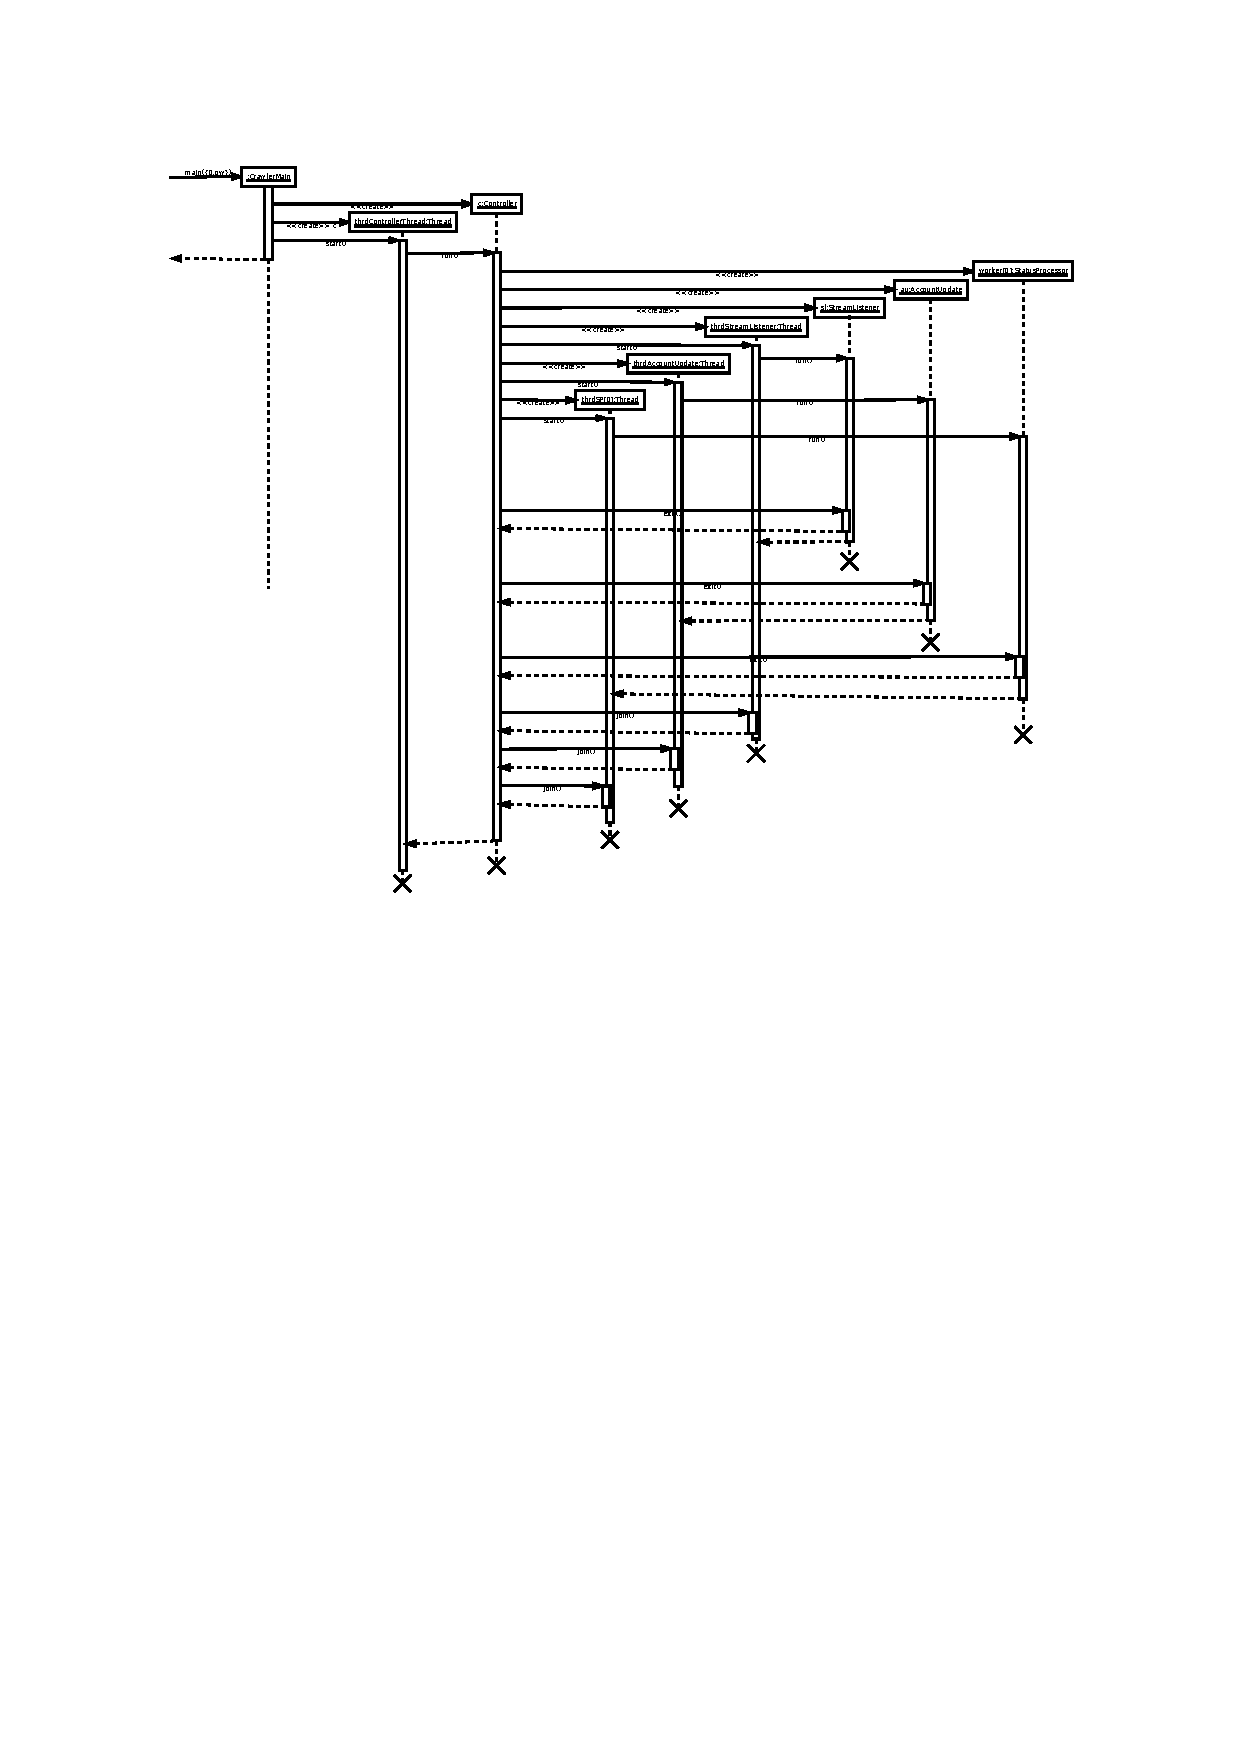
\includegraphics[width=\textheight,height=\textwidth,keepaspectratio=true,angle=-90]{dia/crawler_start_sequence}
	\caption{Sequenzdiagramm zum Start des Crawlers}
	\label{fig:crawler_start}
\end{figure}

\subsection{Verarbeitung der Daten von Twitter}
Um zu verdeutlichen wie die Daten von Twitter innerhalb des Crawlers verarbeitet werden, ist in \cref{fig:crawler_process} der Datenfluss durch den Crawler exemplarisch dargestellt. Dabei werden die Daten von Twitter abgeholt, gepuffert, dann gefiltert und schlussendlich in die Datenbank geschrieben.
\begin{figure}[h!]
	\centering
	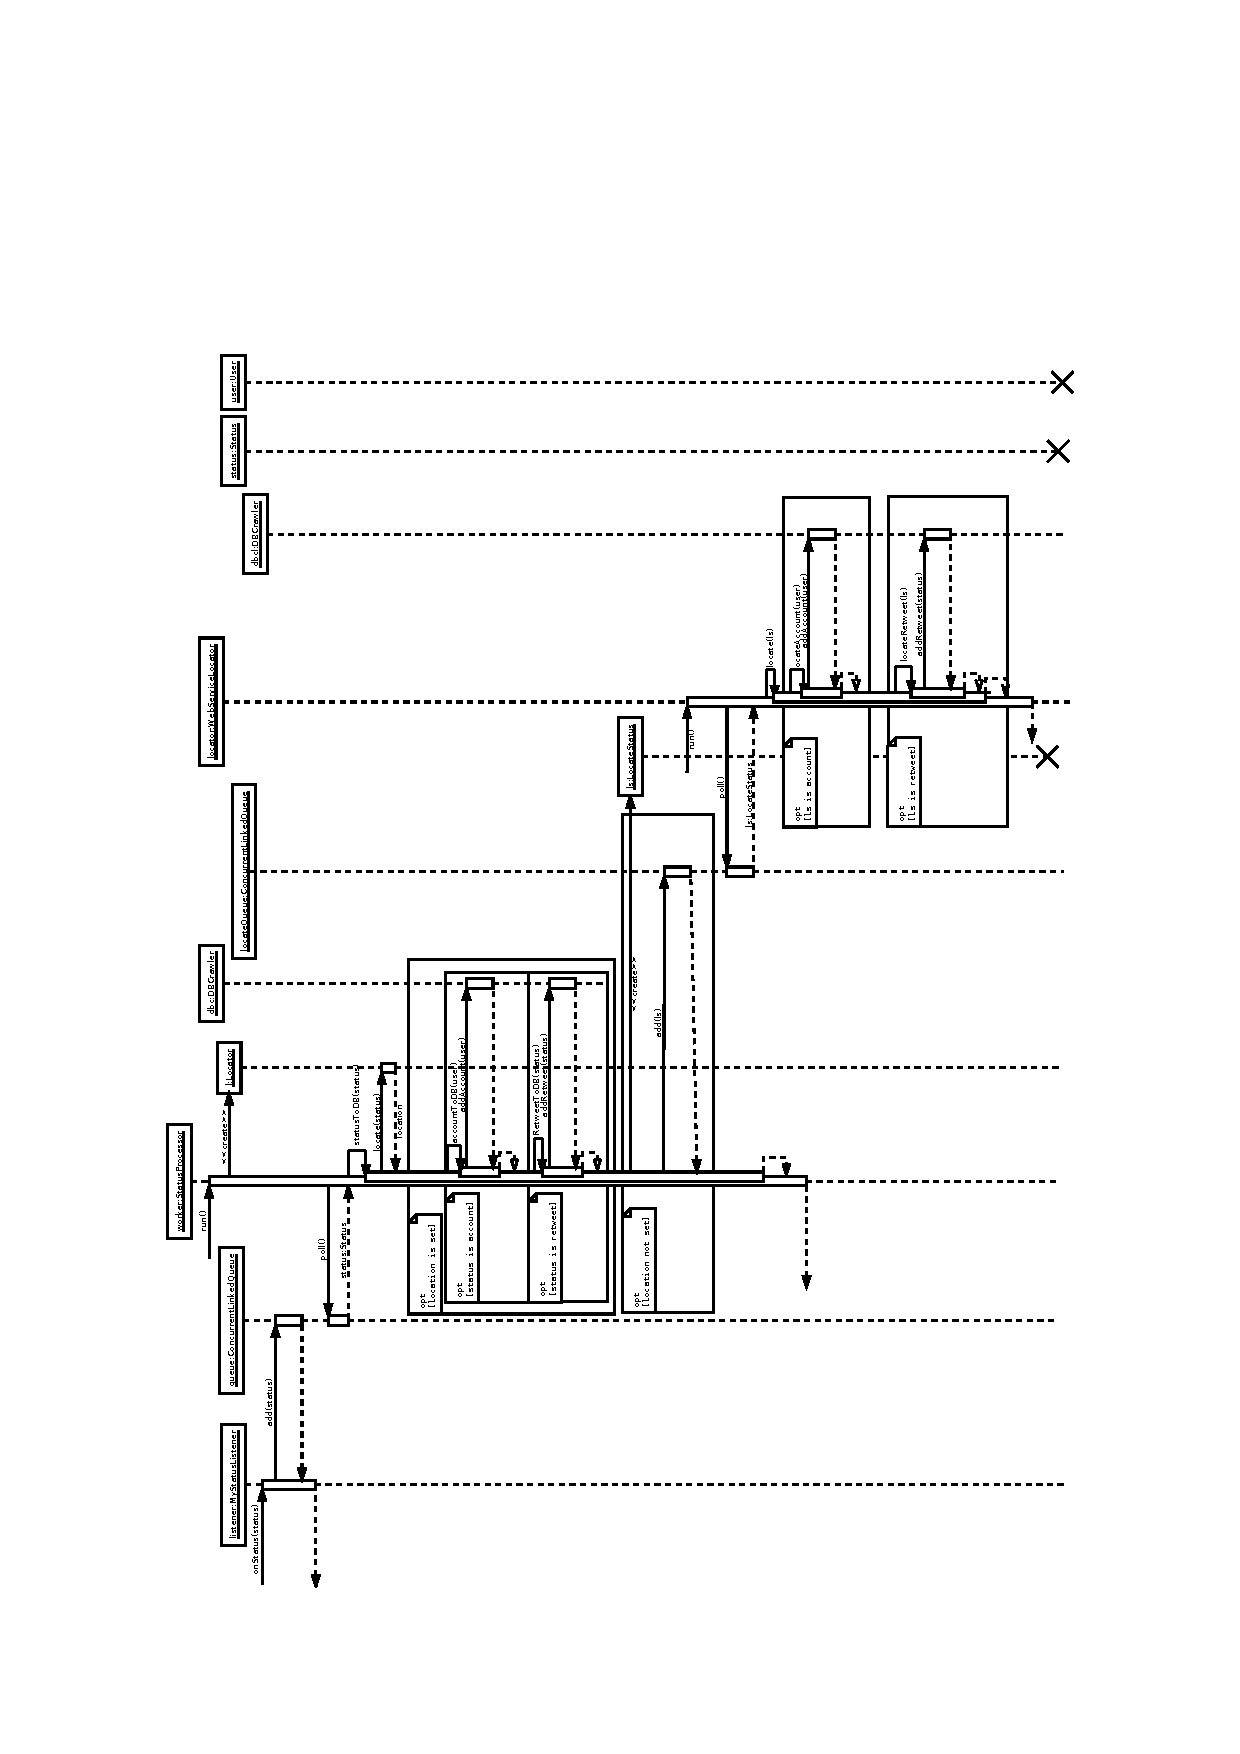
\includegraphics[width=\textheight,height=\textwidth,keepaspectratio=true,angle=-90]{dia/crawler_process_sequence}
	\caption{Sequenzdiagramm der Verarbeitung der Daten von Twitter}
	\label{fig:crawler_process}
\end{figure}

\section{Kategorisierer}

\subsection{Start des Kategorisierers}
Der Kategorisierer soll in regelmäßigen Abständen vom Betriebssystem gestartet werden und daraufhin die neu gefundenen Accounts kategorisieren.

Der Ablauf des Kategorsierers ist im Sequenzdiagramm \ref{fig:categorizerSeq} zu sehen.
\begin{figure}[h!]
	\centering
	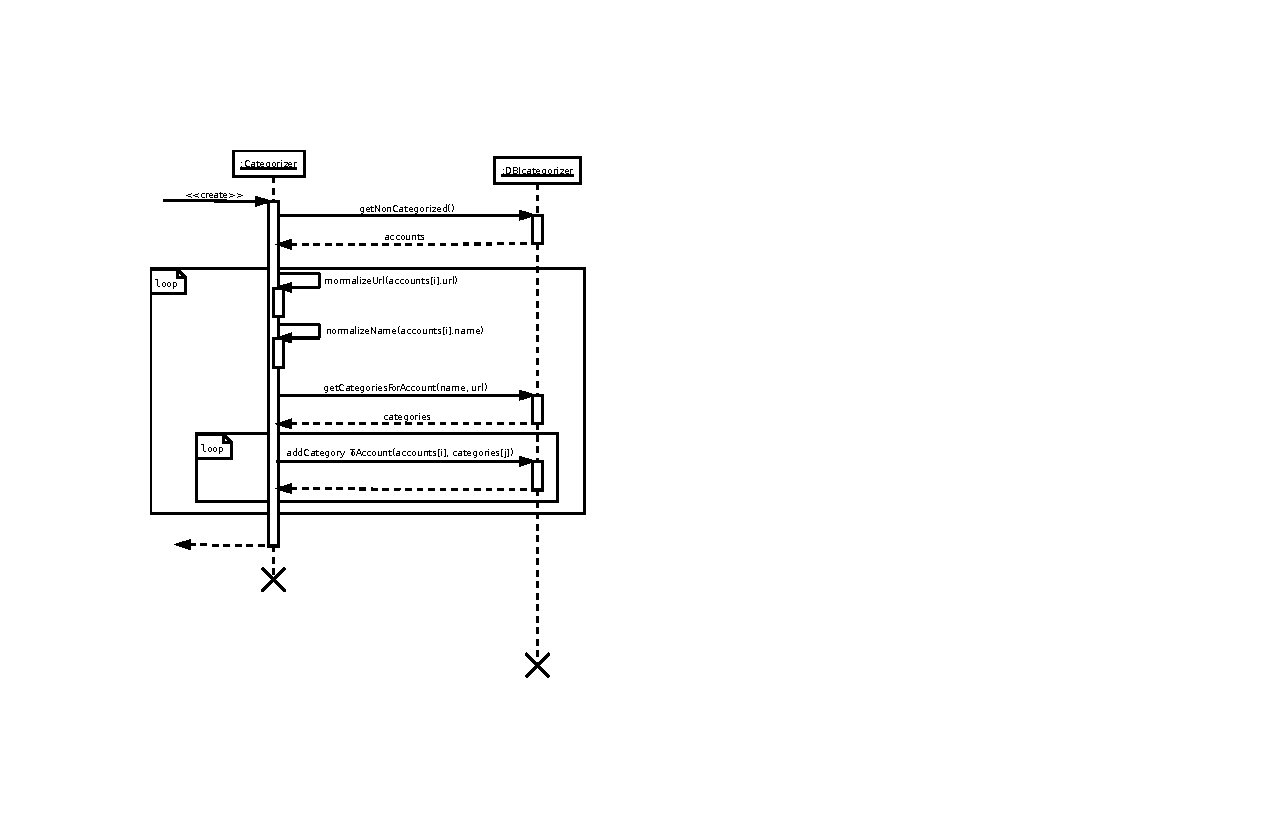
\includegraphics[width=\textwidth,height=\textheight,keepaspectratio=true]{dia/categorizerSequence}
	\caption{Sequenzdiagramm für einen Durchlauf des Kategorisierers. Dabei sind exemplarisch nur jeweils der erste unkategorisierte Account und die erste gefundene Kategorie aufgeführt.}
	\label{fig:categorizerSeq}
\end{figure}

Im ersten Schritt wird also eine Liste von unkategorisierten Accounts ausgelesen. Für jeden dieser Acounts wird eine Liste passender Kategorien ermittelt, die dann nach und nach in die Datenbank geschrieben werden.
\section{GUI}
\begin{figure}[h!]
	\centering
	\includegraphics[width=\textheight,height=\textwidth,keepaspectratio=true,angle=-90]{dia/TwitterGUI_Erweiterung_SequenzDiagramm}
	\caption{Sequenzdiagramm für Auswahl einer neuen Kategorie in der GUI.}
	\label{fig:GUISeq}
\end{figure}
